\begin{figure}[H]
	\centering
	\caption{Considerações iniciais de corpo/sólido.}
	\vspace*{5mm}
	

\tikzset{every picture/.style={line width=0.75pt}} %set default line width to 0.75pt        

\begin{tikzpicture}[x=0.75pt,y=0.75pt,yscale=-1,xscale=1]
%uncomment if require: \path (0,263); %set diagram left start at 0, and has height of 263

%Shape: Polygon Curved [id:ds3141906788381823] 
\draw  [fill={rgb, 255:red, 0; green, 27; blue, 255 }  ,fill opacity=0.4 ] (222.42,99.55) .. controls (239.91,67.75) and (341.68,45.49) .. (342.48,90.33) .. controls (343.27,135.17) and (310.67,138.03) .. (342.48,185.73) .. controls (374.28,233.44) and (244.69,252.2) .. (214.47,198.14) .. controls (184.26,144.07) and (204.93,131.35) .. (222.42,99.55) -- cycle ;
%Straight Lines [id:da6314952819831736] 
\draw    (280.8,132.17) -- (360.61,109.62) ;
\draw [shift={(363.5,108.8)}, rotate = 524.22] [fill={rgb, 255:red, 0; green, 0; blue, 0 }  ][line width=0.08]  [draw opacity=0] (8.93,-4.29) -- (0,0) -- (8.93,4.29) -- cycle    ;
%Shape: Square [id:dp6686503118466058] 
\draw   (273,129.37) -- (283,129.37) -- (283,139.37) -- (273,139.37) -- cycle ;
%Straight Lines [id:da9703547893662439] 
\draw    (283,139.37) -- (288,134.37) ;
%Straight Lines [id:da25502611047122703] 
\draw    (278,124.37) -- (273,129.37) ;
%Straight Lines [id:da37300180195069665] 
\draw    (283,129.37) -- (288,124.37) ;
%Shape: Polygon Curved [id:ds29380683089138615] 
\draw   (323.71,190.28) .. controls (336.43,190.91) and (353.61,185.82) .. (345.98,207.45) .. controls (333.89,237.34) and (261.38,233.53) .. (237.85,219.54) .. controls (214.31,205.54) and (243.25,205.72) .. (255.66,200.45) .. controls (269.65,197.27) and (282.37,195.37) .. (290.64,194.09) .. controls (300.82,193.46) and (310.36,191.55) .. (323.71,190.28) -- cycle ;
%Straight Lines [id:da1546964886690403] 
\draw    (265.87,197.8) -- (248.53,224.44) ;
%Straight Lines [id:da8509460340636961] 
\draw    (276.27,196.2) -- (257.33,227.24) ;
%Straight Lines [id:da7188079684530817] 
\draw    (287.47,193.8) -- (266.27,228.6) ;
%Straight Lines [id:da7809751807828349] 
\draw    (297.87,193) -- (274.67,229.8) ;
%Straight Lines [id:da08571927720865924] 
\draw    (307.71,191.8) -- (283.07,231) ;
%Straight Lines [id:da5493174040388322] 
\draw    (318.27,190.2) -- (292.67,230.6) ;
%Straight Lines [id:da8085612466896939] 
\draw    (327.71,189.8) -- (302.27,229.8) ;
%Straight Lines [id:da9523630969124384] 
\draw    (336.67,189.8) -- (311.07,229.4) ;
%Straight Lines [id:da6401638532153577] 
\draw    (344.27,191.4) -- (322.27,226.2) ;
%Straight Lines [id:da24954550704166478] 
\draw    (347.47,200.2) -- (334.67,219.8) ;
%Straight Lines [id:da943380168411545] 
\draw    (253.87,200.95) -- (240.67,221.4) ;
%Straight Lines [id:da4257592720050687] 
\draw    (244.44,203.24) -- (234.15,217.24) ;
%Straight Lines [id:da06291407970410123] 
\draw    (278,124.37) -- (288,124.37) ;
%Straight Lines [id:da282253289894145] 
\draw    (288,134.37) -- (288,124.37) ;
%Curve Lines [id:da33711672485429256] 
\draw    (277.73,89.27) .. controls (281.4,86.27) and (282.13,85.84) .. (289.73,85.27) ;
%Curve Lines [id:da44596307545388725] 
\draw    (286.9,97.27) .. controls (290.57,94.27) and (291.3,93.84) .. (298.9,93.27) ;
%Curve Lines [id:da41326836388188637] 
\draw    (282.4,93.27) .. controls (286.07,90.27) and (286.8,89.84) .. (294.4,89.27) ;
%Straight Lines [id:da3457855300007193] 
\draw    (287,40.5) -- (287,87.5) ;
\draw [shift={(287,90.5)}, rotate = 270] [fill={rgb, 255:red, 0; green, 0; blue, 0 }  ][line width=0.08]  [draw opacity=0] (8.93,-4.29) -- (0,0) -- (8.93,4.29) -- cycle    ;
%Curve Lines [id:da2439420294185104] 
\draw    (322.27,226.2) .. controls (332.97,238.37) and (347.87,242.97) .. (376.32,232.06) ;
\draw [shift={(379,231)}, rotate = 517.9200000000001] [fill={rgb, 255:red, 0; green, 0; blue, 0 }  ][line width=0.08]  [draw opacity=0] (8.93,-4.29) -- (0,0) -- (8.93,4.29) -- cycle    ;
%Curve Lines [id:da0026897668284329157] 
\draw    (309,161) .. controls (319.81,150.48) and (335.09,174.33) .. (356.63,162.44) ;
\draw [shift={(359,161)}, rotate = 506.48] [fill={rgb, 255:red, 0; green, 0; blue, 0 }  ][line width=0.08]  [draw opacity=0] (8.93,-4.29) -- (0,0) -- (8.93,4.29) -- cycle    ;

% Text Node
\draw (367,94.77) node [anchor=north west][inner sep=0.75pt]    {$\vt{b} \ \text{(forças de volume)}$};
% Text Node
\draw (99.67,142.44) node [anchor=north west][inner sep=0.75pt]    {$\delta _{f} \cup \delta _{u} =\Gamma $};
% Text Node
\draw (290.2,32.8) node [anchor=north west][inner sep=0.75pt]    {$\vt{t} \ \text{(forças de superfície)}$};
% Text Node
\draw (385,220.4) node [anchor=north west][inner sep=0.75pt]    {$\delta _{u} \ \text{(deslocamentos prescritos)}$};
% Text Node
\draw (362,153.4) node [anchor=north west][inner sep=0.75pt]    {$\delta _{f} \ \text{(forças prescritas)}$};
% Text Node
\draw (92,104.4) node [anchor=north west][inner sep=0.75pt]    {$\text{corpo}\rightarrow \text{sólido}$};


\end{tikzpicture}

\end{figure}

\begin{itemize}
	\item Configuração do sólido: posição ocupada pelos pontos em um determinado instante $t$;
	\item Descrever a configuração deformada ($V$) a partir de uma configuração de referência ($V^r$);
	\item \sloppy Considerando um conjunto de pontos da Geometria Euclidiana ($E$), e seja, $(\vt{e}_1,\;\vt{e}_2,\;\vt{e}_3)$ uma base do espaço vetorial da geometria clássica.
\end{itemize}
	
Podemos definir $(0,\;\vt{e}_1,\;\vt{e}_2,\;\vt{e}_3)$ como um sistema de referência:

\begin{figure}[H]
	\centering
	\caption{Campo de deslocamentos.}
	

\tikzset{every picture/.style={line width=0.75pt}} %set default line width to 0.75pt        

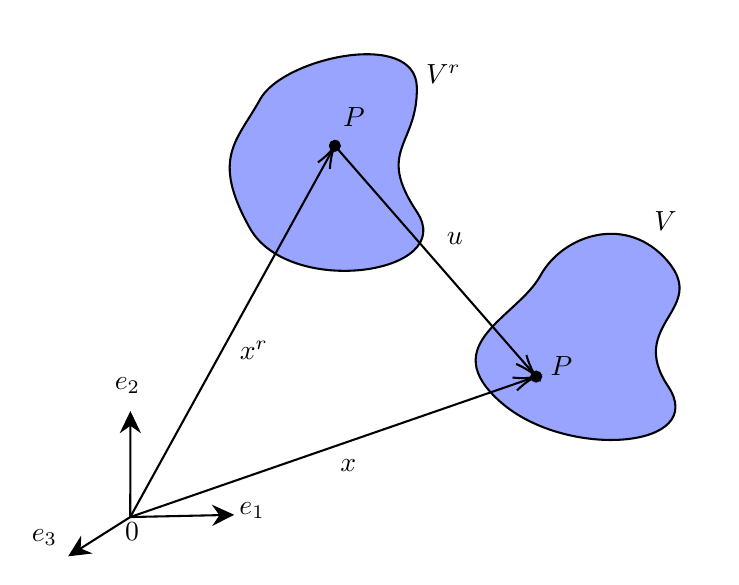
\begin{tikzpicture}[x=0.75pt,y=0.75pt,yscale=-1,xscale=1]
%uncomment if require: \path (0,264); %set diagram left start at 0, and has height of 264

%Shape: Polygon Curved [id:ds23301958927076183] 
\draw  [fill={rgb, 255:red, 0; green, 27; blue, 255 }  ,fill opacity=0.4 ] (132.5,31.7) .. controls (143.5,11.7) and (207.5,-2.3) .. (208,25.9) .. controls (208.5,54.1) and (188,55.9) .. (208,85.9) .. controls (228,115.9) and (146.5,127.7) .. (127.5,93.7) .. controls (108.5,59.7) and (121.5,51.7) .. (132.5,31.7) -- cycle ;
%Shape: Polygon Curved [id:ds07650390385014516] 
\draw  [fill={rgb, 255:red, 0; green, 27; blue, 255 }  ,fill opacity=0.4 ] (267.5,116.7) .. controls (278.5,96.7) and (309.5,86.7) .. (329,109.9) .. controls (348.5,133.1) and (309,139.9) .. (329,169.9) .. controls (349,199.9) and (280.5,205.7) .. (248.5,177.7) .. controls (216.5,149.7) and (256.5,136.7) .. (267.5,116.7) -- cycle ;
%Straight Lines [id:da5659027756383297] 
\draw    (69.92,232.98) -- (263.61,165.96) ;
\draw [shift={(265.5,165.3)}, rotate = 520.9100000000001] [color={rgb, 255:red, 0; green, 0; blue, 0 }  ][line width=0.75]    (10.93,-3.29) .. controls (6.95,-1.4) and (3.31,-0.3) .. (0,0) .. controls (3.31,0.3) and (6.95,1.4) .. (10.93,3.29)   ;
%Shape: Circle [id:dp33072264254260797] 
\draw  [fill={rgb, 255:red, 0; green, 0; blue, 0 }  ,fill opacity=1 ] (166.1,54.1) .. controls (166.1,52.78) and (167.17,51.7) .. (168.5,51.7) .. controls (169.83,51.7) and (170.9,52.78) .. (170.9,54.1) .. controls (170.9,55.43) and (169.83,56.5) .. (168.5,56.5) .. controls (167.17,56.5) and (166.1,55.43) .. (166.1,54.1) -- cycle ;
%Shape: Circle [id:dp6820829798134418] 
\draw  [fill={rgb, 255:red, 0; green, 0; blue, 0 }  ,fill opacity=1 ] (263.1,165.3) .. controls (263.1,163.98) and (264.17,162.9) .. (265.5,162.9) .. controls (266.83,162.9) and (267.9,163.98) .. (267.9,165.3) .. controls (267.9,166.63) and (266.83,167.7) .. (265.5,167.7) .. controls (264.17,167.7) and (263.1,166.63) .. (263.1,165.3) -- cycle ;
%Straight Lines [id:da5268734143852947] 
\draw    (69.92,232.98) -- (167.53,55.85) ;
\draw [shift={(168.5,54.1)}, rotate = 478.86] [color={rgb, 255:red, 0; green, 0; blue, 0 }  ][line width=0.75]    (10.93,-3.29) .. controls (6.95,-1.4) and (3.31,-0.3) .. (0,0) .. controls (3.31,0.3) and (6.95,1.4) .. (10.93,3.29)   ;
%Straight Lines [id:da4223642623796222] 
\draw    (168.5,54.1) -- (264.19,163.8) ;
\draw [shift={(265.5,165.3)}, rotate = 228.9] [color={rgb, 255:red, 0; green, 0; blue, 0 }  ][line width=0.75]    (10.93,-3.29) .. controls (6.95,-1.4) and (3.31,-0.3) .. (0,0) .. controls (3.31,0.3) and (6.95,1.4) .. (10.93,3.29)   ;
%Straight Lines [id:da15852304301408338] 
\draw    (69.92,232.98) -- (70,184.9) ;
\draw [shift={(70,181.9)}, rotate = 450.09] [fill={rgb, 255:red, 0; green, 0; blue, 0 }  ][line width=0.08]  [draw opacity=0] (10.72,-5.15) -- (0,0) -- (10.72,5.15) -- (7.12,0) -- cycle    ;
%Straight Lines [id:da35641451568895] 
\draw    (69.92,232.98) -- (117,231.97) ;
\draw [shift={(120,231.9)}, rotate = 538.76] [fill={rgb, 255:red, 0; green, 0; blue, 0 }  ][line width=0.08]  [draw opacity=0] (10.72,-5.15) -- (0,0) -- (10.72,5.15) -- (7.12,0) -- cycle    ;
%Straight Lines [id:da5944288129967534] 
\draw    (69.92,232.98) -- (42.54,250.3) ;
\draw [shift={(40,251.9)}, rotate = 327.69] [fill={rgb, 255:red, 0; green, 0; blue, 0 }  ][line width=0.08]  [draw opacity=0] (10.72,-5.15) -- (0,0) -- (10.72,5.15) -- (7.12,0) -- cycle    ;

% Text Node
\draw (121,224.3) node [anchor=north west][inner sep=0.75pt]    {$\vt{e}_{1}$};
% Text Node
\draw (169.71,203.74) node [anchor=north west][inner sep=0.75pt]    {$\vt{x}$};
% Text Node
\draw (121.21,146.94) node [anchor=north west][inner sep=0.75pt]    {$\vt{x}^{r}$};
% Text Node
\draw (211,13.3) node [anchor=north west][inner sep=0.75pt]    {$V^{r}$};
% Text Node
\draw (321,84.3) node [anchor=north west][inner sep=0.75pt]    {$V$};
% Text Node
\draw (61,164.3) node [anchor=north west][inner sep=0.75pt]    {$\vt{e}_{2}$};
% Text Node
\draw (21,237.3) node [anchor=north west][inner sep=0.75pt]    {$\vt{e}_{3}$};
% Text Node
\draw (271,154.3) node [anchor=north west][inner sep=0.75pt]    {$P$};
% Text Node
\draw (171,34.3) node [anchor=north west][inner sep=0.75pt]    {$P$};
% Text Node
\draw (221,94.3) node [anchor=north west][inner sep=0.75pt]    {$\vt{u}$};
% Text Node
\draw (66,234.3) node [anchor=north west][inner sep=0.75pt]    {$0$};


\end{tikzpicture}

\end{figure}
	
Os vetores dos pontos de referência ($\vt{x}^r$) e na configuração deformada ($\vt{x}$) em relação aos versores da base podem ser expressos na notação de Einstein:

\[\vt{x}^r=\vt{x}^r-\vt{0}=\sum_{i=1}^3x^{ri}e_i=x^{r1}\vt{e}_1+x^{r2}\vt{e}_2+x^{r3}\vt{e}_3\]
\[\vt{x}=\vt{x}-\vt{0}=\sum_{i=1}^3x^ie_i=x^1\vt{e}_1+x^2\vt{e}_2+x^3\vt{e}_3\]

Seja $f$ uma função que associa a posição de cada ponto na configuração $V^r$ a sua posição na configuração $V$. Tal aplicação é uma transformação de $V^r$ em $V$.
	
\[x^1=\hat{f}_1(x^{r1},\;x^{r2},\;x^{r3})\]
\[x^2=\hat{f}_2(x^{r1},\;x^{r2},\;x^{r3})\]
\[x^3=\hat{f}_3(x^{r1},\;x^{r2},\;x^{r3})\]

Aqui, o circunflexo denota \textit{em função de}, \textit{i.e.}, a coordenada $i$ da posição deformada está em função das coordenadas da posição de referência.
	
Exemplo: Considere um sólido cuja seção no plano $\vt{e}_1$, $\vt{e}_2$ é dado por:
	
//Inserir imagem
	
Caracterize os seguintes campos de deslocamento:
	
\begin{enumerate}[a)]
	\item Translação de corpo rígido de intensidade $\Delta$ na direção de $\vt{e}_1$;
	\item Rotação de corpo rígido em torno de $\vt{e}_3$ de intensidade $\varphi$.
\end{enumerate}
	
Resolução:
	
\begin{enumerate}[a)]
	\item
		\[
		\vt{u}=
			\begin{Bmatrix}
			u_1 \\ u_2 \\ u_3
			\end{Bmatrix}
			=
			\begin{Bmatrix}
				\Delta \\ 0 \\ 0
			\end{Bmatrix}
		\]
		\[\vt{u}=\vt{x}-\vt{x}^r
		\implies
		\vt{x}=
		\begin{cases} x^1=x^{r1}+u_1=x^{r1}+\Delta \\ x^2=x^{r2}+u_2=x^{r2} \\ x^3=x^{r3}+u_3=x^{r3}
		\end{cases}
		\]
	\item
		//Inserir imagem
			
		A configuração de referência:
		\[x^{r1}=r\cdot \cos\theta\]
		\[x^{r2}=r\cdot\sin\theta\]
		\[x^{r3}=0\;\text{(ou }x^{r3}\text{ para deixar genérico})\]
			
		A configuração deformada (a partir da imagem):
			
		\[u^1=r\cdot\cos(\varphi+\theta)-r\cdot\cos\theta\]
		\[u^1=r\cdot\cos\varphi\cdot\cos\theta-r\cdot\sin\varphi\cdot\sin\theta-r\cdot\cos\theta\]
			
		\[u^2=r\cdot\sin(\varphi+\theta)-r\cdot\sin\theta\]
		\[u^2=r\cdot\sin\varphi\cdot\cos\theta+r\cdot\sin\theta\cdot\cos\varphi-r\cdot\sin\theta\]
			
		Substituindo as coordenadas de referência nas coordenadas deformadas:

		\[u^1=x^{r1}\cdot\cos\varphi-x^{r2}\cdot\sin\varphi-x^{r1}\]
		\[u^2=x^{r1}\cdot\sin\varphi+x^{r2}\cdot\cos\varphi-x^{r2}\]
		\[u^3=0\]
			
		Como sabemos que $\vt{x}=\vt{x}^r+\utilde{\mathbf{u}}$, temos:
			
		\[
			\begin{cases}
				x^1=x^{r1}\cdot\cos\varphi-x^{r2}\cdot\sin\varphi \\ x^2=x^{r1}\cdot\sin\varphi+x^{r2}\cdot\cos\varphi \\ x^3=x^{r3}
			\end{cases}
		\]
			
		Podemos escrever também na forma matricial:
			
		\[
			\begin{Bmatrix}
				x^1 \\ x^2 \\ x^3
			\end{Bmatrix}
			=
			\begin{bmatrix}	
				\cos\varphi & -\sin\varphi & 0 \\
				\sin\varphi & \cos\varphi & 0 \\
				0 & 0 & 1
			\end{bmatrix}
			\begin{Bmatrix}
				x^{r1} \\ x^{r2} \\ x^{r3}
			\end{Bmatrix}							
		\]
\end{enumerate}